\documentclass{article}
\usepackage[utf8]{inputenc}
\usepackage{geometry}


\usepackage{amsmath}
\usepackage{booktabs}
\usepackage{array}
\usepackage{hyperref}
\usepackage{minted}
\usepackage{float}

\geometry{
  a4paper,
  total={170mm,257mm},
  left=20mm,
  top=20mm,
}

\usepackage{graphicx}
\usepackage{titling}

\title{Occupancy Mapping of Indoor Environment Using P3DX Robot\\
and Ultrasonic Sensors in CoppeliaSim}
\date{20 May 2026}

\usepackage{fancyhdr}
\fancypagestyle{plain}{%
    \fancyhf{}
    \fancyfoot[R]{}
    \fancyfoot[L]{}
    \fancyhead[L]{
\includegraphics[width=2cm]{ITS_pojok.pdf}}
    \fancyhead[R]{\today}
}
\makeatletter
\def\@maketitle{%
  \newpage
  \null
  \vskip 1em%
  \begin{center}%
  \let \footnote \thanks
    {\LARGE \@title \par}%
    \vskip 1em%
  \end{center}%
  \par
  \vskip 1em}
\makeatother

\usepackage{lipsum}

\begin{document}

\maketitle

\noindent\begin{tabular}{@{}ll}
    Author(s):          & Muhammad Bari Akmal \\
    Teacher:            & Muhammad Qomaruz Zaman, S.T., M.T., Ph.D. \\
    Class name:         & Sistem Robot Otonom \\
    YouTube video link: & \url{https://youtu.be/XYKgtL1H1vo} \\
    GitHub link:        & \url{https://github.com/Drimal-835/Otomation-of-Robotic-System}
\end{tabular}
\vspace{2cm}

Pada tugas ini, digunakan model robot P3DX sebagai objek simulasi dan CoppeliaSim sebagai
aplikasi untuk melakukan simulasi. Tujuan dari tugas ini adalah melakukan pemetaan
(\textit{mapping}) lingkungan dalam ruangan menggunakan empat sensor ultrasonik yang terpasang
pada robot P3DX. Robot bergerak secara otomatis menggunakan algoritma Braitenberg bawaan
CoppeliaSim, sementara kode Python membaca data sensor dan mencatat titik-titik hambatan ke
dalam frame dunia (\textit{world frame}). Peta akan ditampilkan setelah simulasi selesai.

\section*{Lingkungan Simulasi (Actual Map)}

Gambar~\ref{fig:actual_map} menunjukkan tampilan atas lingkungan simulasi yang digunakan
dalam CoppeliaSim. Lingkungan ini merupakan ruang kelas B202 yang berisi meja, kursi, dan
dinding pembatas.

\begin{figure}[H]
    \centering
    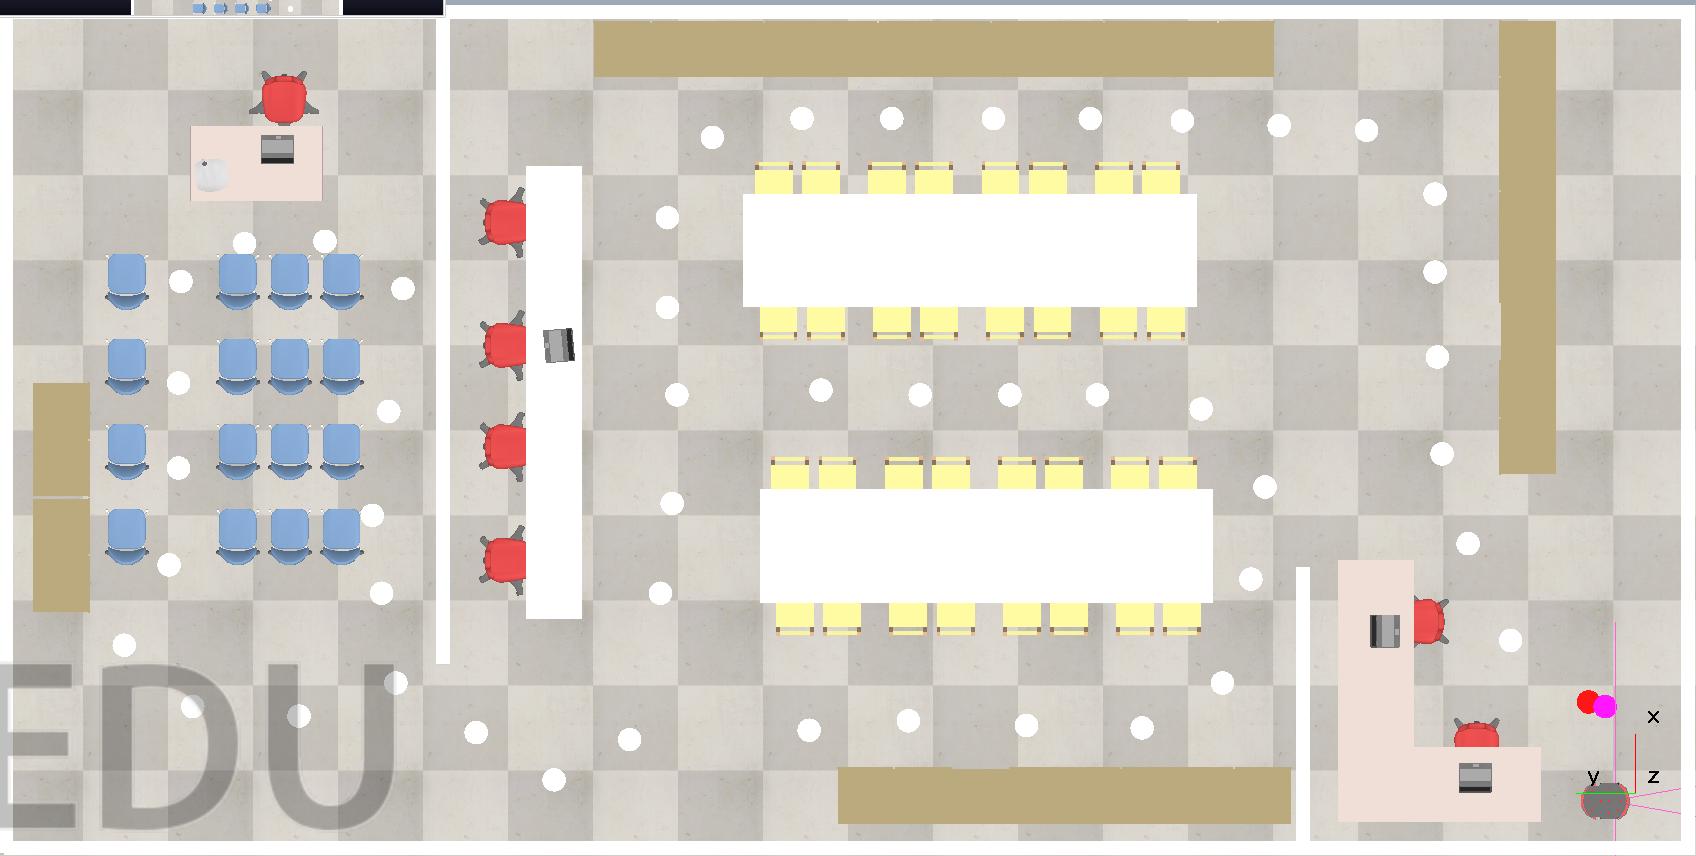
\includegraphics[width=0.95\linewidth]{coppelia_scene.png}
    \caption{Tampilan atas lingkungan simulasi B202 di CoppeliaSim (Actual Map)}
    \label{fig:actual_map}
\end{figure}

\section*{Hasil Pemetaan (Mapping Result)}

Gambar~\ref{fig:mapping_result} menunjukkan hasil pemetaan yang diperoleh dari pembacaan
keempat sensor ultrasonik (indeks 0, 3, 4, dan 7) selama robot bergerak mengelilingi
lingkungan. Setiap titik pada grafik merepresentasikan satu deteksi hambatan yang telah
ditransformasikan ke dalam frame dunia menggunakan matriks transformasi homogen.

\begin{figure}[H]
    \centering
    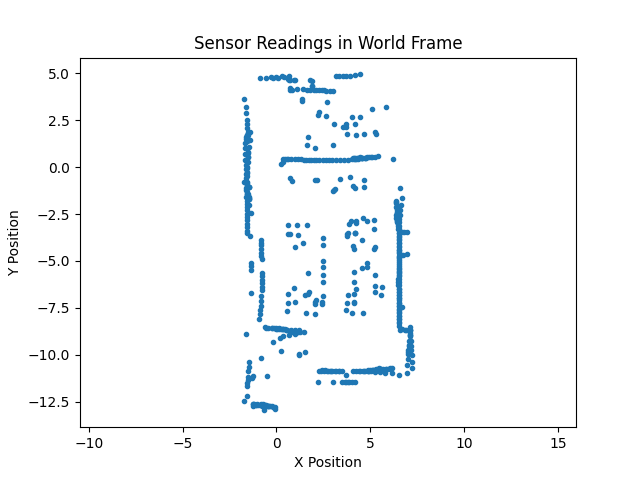
\includegraphics[width=0.75\linewidth]{b202_map.png}
    \caption{Hasil pemetaan sensor ultrasonik P3DX dalam world frame}
    \label{fig:mapping_result}
\end{figure}

\section*{Kode Python}

Berikut adalah kode Python yang digunakan untuk melakukan pemetaan menggunakan empat sensor
ultrasonik (indeks 0, 3, 4, dan 7). Kode ini terhubung ke CoppeliaSim melalui ZMQ Remote
API, membaca posisi robot dan titik deteksi sensor, mentransformasikan setiap titik ke dalam
frame dunia, dan menampilkan peta setelah simulasi berhenti.

\begin{minted}[frame=lines, framesep=2mm, linenos, breaklines]{python}
import time
import math
import numpy as np
import matplotlib.pyplot as plt
from coppeliasim_zmqremoteapi_client import RemoteAPIClient


def transformMat(alpha, beta, gamma, tx, ty, tz):
    rotx = np.array([
        [1, 0, 0],
        [0, math.cos(alpha), -math.sin(alpha)],
        [0, math.sin(alpha),  math.cos(alpha)]
    ])
    roty = np.array([
        [ math.cos(beta), 0, math.sin(beta)],
        [0, 1, 0],
        [-math.sin(beta), 0, math.cos(beta)]
    ])
    rotz = np.array([
        [math.cos(gamma), -math.sin(gamma), 0],
        [math.sin(gamma),  math.cos(gamma), 0],
        [0, 0, 1]
    ])
    rot_total = np.matmul(np.matmul(rotx, roty), rotz)
    trans_vector = np.array([[tx], [ty], [tz]])
    R_t_3x4 = np.hstack((rot_total, trans_vector))
    homogeneous_row = np.array([[0, 0, 0, 1]])
    return np.vstack((R_t_3x4, homogeneous_row))


# 1. Connect
client = RemoteAPIClient()
sim = client.require('sim')

# 2. Start simulation
sim.startSimulation()
print("Simulation started.")
sim.addLog(1, "Mapping started from Python!")

# 3. Get handles
p3dx = sim.getObject("/PioneerP3DX")

SENSOR_INDICES = [0, 3, 4, 7]   # 0-based indices matching the Lua script
sensor_handles = []
for idx in SENSOR_INDICES:
    h = sim.getObject("/ultrasonicSensor", {"index": idx})
    sensor_handles.append(h)

# 4. Storage
hits_x = {idx: [] for idx in SENSOR_INDICES}
hits_y = {idx: [] for idx in SENSOR_INDICES}
path_x, path_y = [], []

# 5. Main loop
RUN_SECONDS = 60

try:
    start_time = time.time()
    step = 0
    while (time.time() - start_time) < RUN_SECONDS:
        elapsed = time.time() - start_time
        print(f"  t={elapsed:.1f}s", end="\r")

        # Robot pose in world frame
        p3dx_pos = sim.getObjectPosition(p3dx, sim.handle_world)
        p3dx_ori = sim.getObjectOrientation(p3dx, sim.handle_world)
        path_x.append(p3dx_pos[0])
        path_y.append(p3dx_pos[1])

        T_body_world = transformMat(
            p3dx_ori[0], p3dx_ori[1], p3dx_ori[2],
            p3dx_pos[0], p3dx_pos[1], p3dx_pos[2]
        )

        for i, (idx, h) in enumerate(zip(SENSOR_INDICES, sensor_handles)):
            res, dist, prox_point, prox_obj, prox_n = \
                sim.readProximitySensor(h)

            if res and dist > 0:
                # Use prox_point: actual hit XYZ in sensor local frame
                sensor_hit = np.array([
                    [prox_point[0]],
                    [prox_point[1]],
                    [prox_point[2]],
                    [1]
                ])

                # Sensor pose relative to robot body
                s_pos = sim.getObjectPosition(h, p3dx)
                s_ori = sim.getObjectOrientation(h, p3dx)
                T_sensor_body = transformMat(
                    s_ori[0], s_ori[1], s_ori[2],
                    s_pos[0], s_pos[1], s_pos[2]
                )

                # sensor frame -> body frame -> world frame
                hit_body  = np.matmul(T_sensor_body, sensor_hit)
                hit_world = np.matmul(T_body_world,  hit_body)

                hits_x[idx].append(hit_world[0][0])
                hits_y[idx].append(hit_world[1][0])

        step += 1
        time.sleep(0.02)

finally:
    sim.stopSimulation()
    print("\nSimulation stopped.")

# 6. Plot
all_x = []
all_y = []
for idx in SENSOR_INDICES:
    all_x.extend(hits_x[idx])
    all_y.extend(hits_y[idx])

plt.figure()
plt.plot(all_x, all_y, '.')
plt.xlabel('X Position')
plt.ylabel('Y Position')
plt.title('Sensor Readings in World Frame')
plt.axis('equal')
plt.show()
\end{minted}

\section*{Penjelasan Algoritma}

Algoritma pemetaan yang digunakan bekerja melalui tiga tahap transformasi koordinat:

\begin{enumerate}
    \item \textbf{Frame sensor ke frame robot (body):} Titik deteksi yang dikembalikan oleh
          \texttt{sim.readProximitySensor()} dalam koordinat lokal sensor
          ditransformasikan ke koordinat robot menggunakan matriks transformasi homogen
          $T_{\text{sensor} \to \text{body}}$.

    \item \textbf{Frame robot ke frame dunia (world):} Hasil transformasi pertama kemudian
          ditransformasikan lagi ke frame dunia menggunakan $T_{\text{body} \to \text{world}}$
          yang dibangun dari posisi dan orientasi robot aktual pada setiap langkah waktu.

    \item \textbf{Akumulasi titik:} Semua titik hasil transformasi disimpan dan divisualisasikan
          setelah simulasi selesai menggunakan \texttt{matplotlib}.
\end{enumerate}

Sensor yang digunakan adalah sensor ultrasonik indeks 0, 3, 4, dan 7 (berbasis indeks 0
sesuai skrip Lua bawaan CoppeliaSim), yang masing-masing menghadap ke arah depan-kiri, kiri,
kanan, dan depan-kanan robot. Pergerakan robot sepenuhnya dikendalikan oleh algoritma
Braitenberg pada skrip Lua bawaan CoppeliaSim tanpa modifikasi dari sisi Python.

\end{document}